\documentclass[12pt, a4paper]{report}
\usepackage[left=1.0 in, right=1.0 in, top=1.0 in, bottom=1.0 in]{geometry}
\usepackage{hyperref}
\usepackage{graphicx}
\usepackage{cite}

\begin{document}
\title{SquareX}
\author{Prashant Jalan (11523)\\
Anubhav Bimbisariye (11131)}
\maketitle
\tableofcontents

\chapter{Introduction}
\section{Description}
This is a python based web game which utilizes pygame library for designing the game engine and graphics interface of the game. We shall use pyjs library to use the game as a java module which can be played in any browser. As part of the midterm evaluation, we have completed implementing the game in python.
\section{Functionality}
The game will have an array of points between which the user can click to join two points.Multiple users shall be assigned colors. When a user creates a new line or a box, it shall be displayed in his respective colour. They shall play one after the other to put a line. In case a square is completed, the same user gets another chance.
The user with most number of squares shall win the game.

\chapter{Designing the game engine}
\section{Pygame Module}
Pygame is a set of Python modules designed for writing games. Pygame adds functionality on top of the excellent SDL library. This allows us to create fully featured games and multimedia programs in the python language. Pygame is highly portable and runs on nearly every platform and operating system. Pygame is free. Released under the GPL License, you can create open source, free, freeware, shareware, and commercial games with it.

\section{Game Description}
Our game starts with a start screen in which the user can choose between a small, medium or large grid to play the game. The non trivial part of our code is that we allow the user to create any custom n $\times$ n grid to play the game.In the grid, the user plays against himself. He switches between two colors, red and yellow to play the game.

\section{Code Description}
We make the n $\times$ n grid using the \textit{draw\_line} and \textit{draw\_circle} function. It is initially gray and black color respectively and serves as the gameplay interface. Then, we detect the mouse click and the nearest line, if exists is colored in accordance with the color of the user who is active.If the line is already colored,then nothing happens.Whenever we change the color of the line, we also detect if a square is formed. If  the square is formed, then a circle is drawn in the middle with the same color.

\chapter{Conclusion \& Future work}

\begin{figure}[!t]
\centering
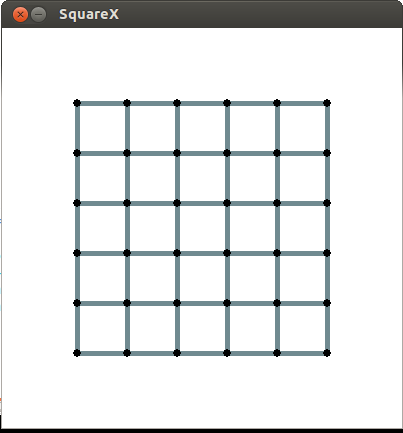
\includegraphics[width=5in]{screenshot.png}
\caption{\small \sl A Screenshot of the game.}
\label{fig_FSM}
\end{figure}

We have been able to make the game. Now we aim to learn the intricacies of implement it in a web server for multiplayer functionality. We also need to learn how we would detect the mouse clicks at different computers connected to the server and incorporate it in our backend programming platform.

\end{document}